% use paper, or submit
% use 11 pt (preferred), 12 pt, or 10 pt only

\documentclass[letterpaper, preprint, paper,11pt]{AAS}	% for preprint proceedings
%\documentclass[letterpaper, paper,11pt]{AAS}		% for final proceedings (20-page limit)
%\documentclass[letterpaper, paper,12pt]{AAS}		% for final proceedings (20-page limit)
%\documentclass[letterpaper, paper,10pt]{AAS}		% for final proceedings (20-page limit)
%\documentclass[letterpaper, submit]{AAS}			% to submit to JAS

\usepackage{bm}
\usepackage{amsmath}
\usepackage{subfigure}
%\usepackage[notref,notcite]{showkeys}  % use this to temporarily show labels
\usepackage[colorlinks=true, pdfstartview=FitV, linkcolor=black, citecolor= black, urlcolor= black]{hyperref}
\usepackage{overcite}
\usepackage{footnpag}			      	% make footnote symbols restart on each page

% https://www.baen.com/rendezvous [1]


\PaperNumber{XX-XXX}



\begin{document}

%%% CHANGE TITLE SEE NOTES%%%%
\title{Model Predictive Control with Sparse Dynamics Identification for Spacecraft Rendezvous}

\author{Daniel Gonzalez\thanks{Engineer, Dynamics and Control Analysis Group, Maxar Space Infrastructure (formerly SSL), 3825 Fabian Way, Palo Alto, CA 94303 U.S.A.},
	 Mohammad Ayoubi\thanks{Associate Professor, Department of Mechanical Engineering, Santa Clara University, 500 El Camino Real,
	 	Santa Clara, CA 95053 U.S.A. AIAA senior member, AAS senior member.} , 
\ and Junette Hsin\thanks{Engineer, Dynamics and Control Analysis Group, Maxar Space Infrastructure (formerly SSL), 3825 Fabian Way, Palo Alto, CA 94303 U.S.A.}, 
}


\maketitle{} 		


\begin{abstract}
	
This paper presents an optimal control solution for the spacecraft rendezvous proximity operations (RPO) problem using dual quaternions. We propose a model predictive control (MPC) law with sparse identification of nonlinear dynamics (SINDY) technique as an identifier to control the attitude and position of a chaser with respect to a target in a circular or elliptical orbit. The proposed MPC minimizes the fuel expenditure in the presence of external disturbances while satisfying actuator constraints. We verify the efficacy and robustness of the proposed controller via numerical simulations.

\end{abstract}








\section{Introduction}
%Paper Title
%Rendezvous Proximity Operations Equations of Motion Derived with SINDy and Controlled with MPC
%
%Problem statement (general)

Space rendezvous missions have been extensively analyzed implementing various forms of constrained path planning and optimization techniques; many of which require high fidelity system identification of the chaser satellite. The combination of improvements in space-certified hardware and modern control techniques have expanded the capability of spacecraft control and the scope of on-orbit services, such as satellite refueling, inspection, and repair, and debris avoidance and removal \cite{ParkZagaris_AnalysisMPC,CairanoPark_MPCRPO}. The increased need and application of these mission types has inspired further research in methods to lower costs, increase fuel savings, and find solutions to rendezvous problems with increasingly complex constraints, all while optimizing for computational efficiency.

One of those well-studied rendezvous methods utilizes model-predictive control (MPC), which has been shown to use less fuel due to minimum-fuel trajectory optimization while finding an optimum seeking approach path within constraints of sensor visibility and safety \cite{RichardsHow_PerformanceMPC}. Richards and How developed and evaluated a new MPC implementation that optimizes using a novel mixed-integer linear programming method. They found fuel saving improvements over traditional MPC methods and the heritage glideslope approach, in which the chaser vehicle
moves along a straight line towards its target. Singh and Bortolami presented an MPC solution to control one of the Space Shuttle's approach phases; their controller optimized the rendezvous path for fuel consumption and constrained the sensor line-of-sight and thruster firing directions to avoid plume impingement. They studied seven real-world cases of the space shuttle's standard orbit raising maneuver on its way to the ISS \cite{SinghBortolami_OptimalMPC}. Cairano and Park shows another example of how an MPC can be used for RPO maneuvers \cite{CairanoPark_MPCRPO}. Their MPC implementation was robust to thrust errors, air drag (low Earth orbit), and solar pressure (geostationary orbits). They optimized considering time-to-dock and fuel consumption while constraining thrust magnitude, line-of-sight, and approach velocity. Kannan and Sajadi-Alamdari apply MPC to spacecraft rendezvous maneuvers while considering fuel-efficiency and collision avoidance in their cost function \cite{KannanAlamdari_MPC}. Park and Zagaris explore collision avoidance during rendezvous operations through both linear and non-linear MPC methods to optimize fuel, limit thrust magnitudes, and operating within safe entry cones\cite{ParkZagaris_AnalysisMPC}. The linear technique uses hyperplanes to convexify obstacles while the nonlinear solution utilizes ellipsoids. The linear method proved to be much more robust, stable, and computationally practical. MPC will be used as the controller in this study because it can optimize the approach path determination for fuel consumption while implementing constraints, but other control methods exist that offer other advantages.

Another scheme that has been used for rendezvous maneuvers is called adaptive control. Filipe and Tsiotras proposed an adaptive position and attitude (pose) tracking controller for proximity operations that requires no knowledge about the mass and inertia of the chaser satellite \cite{FilipeTsiotras_AdaptiveDualQ}. It can also take into account gravitational acceleration, gravity-gradient torque, and other constant disturbance forces and torques, all while in circular or elliptical orbit. This method can perform system identification of the chaser satellite, given that sufficient conditions are met, and then proceed to approach and then dock the target satellite. The controller can handle large time varying errors and is almost globally stable. Finally, given its low order, the algorithm can be used for satellites with limited computational power.

For MPC, adaptive control, and other methods, offline and online system identification techniques are a necessity if high accuracy and precision control is desired, which many times requires costly and expensive volumes of data collection and processing. Within the previously cited adaptive control implementation, Filipe and Tsiotras calculate mass and inertia properties of the system by using known sets of disturbance forces and torques. With this method, the system identification is limited by the measurement quality of the applied forces and torques. Another system identification technique investigated by Kaiser, Kutz, and Brunton that was used with MPC is called sparse identification of nonlinear dynamics (SINDY) \cite{KaiserKutz_SINDyMPC}. SINDY is a data-driven system identification algorithm which can be used to derive governing equations for a nonlinear dynamic systems. In this work, the authors compare SINDY to dynamic mode decomposition (DMD) and a multilayer neural network (NN). They show that sparse identification is preferred when a low volume of noisy data is available and a fast computation time is required. Also, SINDY uncovers the underlying nonlinear dynamic equations of the system, instead of just having a black box that provides little to no physical insight. One of the most useful features of SINDY is that the system identification can be used with control inputs along with other external forcing \cite{BruntonProctor_SINDYc}. It does this all while being fast enough to run on spacecraft embedded systems \cite{ProvostBrunton_SINDyAnalysis}. SINDY does have a few weaknesses, but they can be mitigated. The first is that a sufficient library of functions must be assumed to identify high-dimensional systems \cite{KaiserKutz_SINDyMPC}; this can be prevented by increasing the function library size. Another drawback to this technique is that it does not react effectively to abrupt changes in dynamics, but this concern can be alleviated by using linear methods like DMD while the system dynamics settle.
%%% rewritten 
% FIX CITATIONS 

Robotics and spacecraft rendezvous operations go hand-in-hand, and a powerful tool known as dual quaternions, used mostly with robots, can be brought over to bridge the gap to the on-orbit servicing realm \cite{TsiotrasValverde_DualQTool}. This set of numbers extends the utility found in representing attitude as a quaternion to also describe position and translation. One of the advantages dual quaternions have over quaternion-vector representation is that control laws and dynamics equations can be written in a more compact form \cite{FilipeTsiotras_AdaptiveDualQ,FilipeKontitsis_ExtendedKalmanFilterDualQ}. Pose transformations using dual quaternions are more computationally efficient than the quaternion-vector method \cite{FilipeTsiotras_AdaptiveDualQ,ReynoldsSzmuk_DualQDescent}. There is natural coupling between rotational and translational motion as well as between rotational-only and rotation-translation dual quaternion kinematic equations \cite{FilipeTsiotras_AdaptiveDualQ}. Kinematics for dual quaternions can be easily derived due to multiplicative properties and problems involving kinematic chains can be solved in fewer steps \cite{DooleyMcCarthy_SpatialRBDDualQ}. Controllers or filters developed for attitude quaternions can often be adapted for use with dual quaternions \cite{FilipeTsiotras_AdaptiveDualQ, ValverdeTsiotras_SCRobotDualQ}. Once a controller is adapted, its constraint equations come in a simpler form \cite{DooleyMcCarthy_SpatialRBDDualQ} and its stability can be proven in one step\cite{FilipeTsiotras_AdaptiveDualQ}. Using this number set does come with what some may see as a drawback. For instance, two additional constraint equations are necessary, derived motion relationships can be complicated, physical significance of variables are not initially apparent \cite{DooleyMcCarthy_SpatialRBDDualQ}, there is a quadratic cost on required control commands to minimize propellant use \cite{LeeMesbahi_ConstrainedMPCDualQ}, and they suffer from the so-called unwinding phenomena\cite{FilipeTsiotras_AdaptiveDualQ}.

In this paper, we propose a fuel optimal controller for the rendezvous proximity operations (RPO) problem. We use a dual quaternion formulation of SINDY and MPC to control the position and orientation of the chaser satellite with respect to its target in the presence of external forces while satisfying actuator constraints. 

\section{Dual Quaternion Concept Example}
All dynamics and controls equations discussed in this work are expressed using dual quaternions. We will briefly review how this number set can represent pose via an example. More thorough mathematical properties of quaternions, dual numbers, dual quaternions, and necessary operators are given in Reference \citenum{FilipeTsiotras_AdaptiveDualQ}. 

Within the aerospace industry, single quaternions are used to express the attitude between two reference frames of interest. Combining quaternions with the concept of a dual number $\epsilon$, where $\epsilon^2 = 0$, but $\epsilon \ne 0$, allows the encoding of both rotational and translational information relating two reference frames. Let us consider the chaser and target in the Newtonian frame as shown in Figure \ref{fig:Rel_Pos}. Expressing dual quaternions with a hat symbol, one would express the pose of the chaser with respect to its target as

\begin{figure}[h!]
	\centering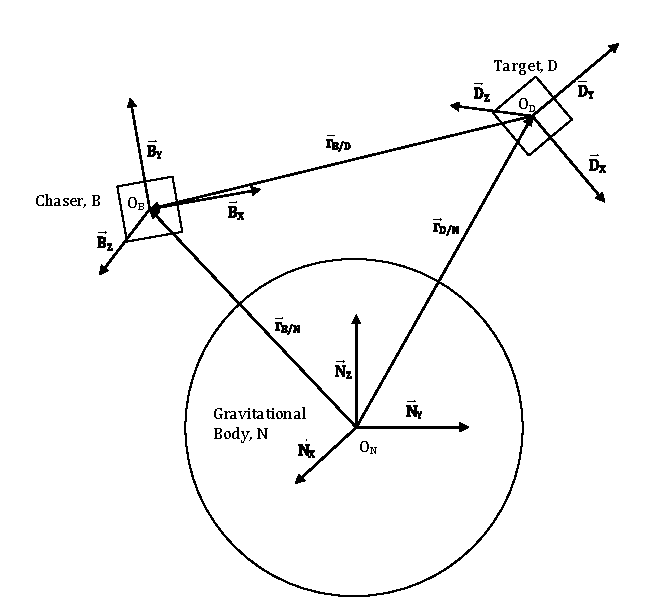
\includegraphics[width=3.5in]{Figures/REL_POSE.pdf}
	\caption{Relative positions between chaser and target spacecraft, orbiting a gravitational body.}
	\label{fig:Rel_Pos}
\end{figure}

\begin{equation}
\begin{aligned}
\label{eq:dual_quat_eg}
\hat{q}_{B/D} = q_{B/D} + \epsilon \frac{1}{2} q_{B/D} r^B_{B/D},
\end{aligned}\\
\end{equation}
where $q_{B/D}$ is the attitude unit quaternion and $r^B_{B/D}$ is the relative position vector of the chaser with respect to the target, in a body fixed basis, represented as a quaternion. Quaternions can be expressed using an ordered pair where the first and second coordinates are the vector and scalar parts, respectively. Using that notation, the attitude is
\begin{equation}
\label{eq:att_quat}
q_{B/D} = (\vec{\mathbf{n}}\sin{(\phi/2)} , \cos{(\phi/2)}) 
\end{equation}
where $\vec{\mathbf{n}}$ is the skew unit vector that one rotates frame D about by $\phi$ to get frame B. The relative position as a quaternion vector-scalar ordered pair is 
\begin{equation}
\label{eq:pos_quat}
r_{B/D}^B = (\vec{\mathbf{r}}_{B/D}^B, 0).
\end{equation}
%Another operator needed to understand the relative motion equation is the dual quaternion conjugation where
%\begin{equation}
%\label{eq:dual_conjugation}
%\hat{q}^* = \hat{q}^*_r + \epsilon\hat{q}^*_d,
%\end{equation}
%assuming $\hat{q}^*_r$ and $\hat{q}^*_d$ are the real and dual parts of $\hat{q}$, and the $*$ operator denotes a quaternion conjugate. The relative dynamics equation also has a 


\section{Relative Dynamic Equations for Rendezvous Proximity Operations}
To simulate relative orbit dynamics and control a satellite using MPC, one must first derive a system model. Assuming quasi-static mass and inertial properties of a chaser spacecraft, B, its motion dynamics relative to a target body, D, are governed by
\begin{equation}
\begin{aligned}
	\label{eq:dyn}
	(\dot{\hat{\omega}}^B_{B/D})^s = (M^B)^{-1}\star(\hat{f}^B-(\hat{\omega}^B_{B/D}+\hat{\omega}^B_{D/N})\times(M^B\star((\hat{\omega}^B_{B/D})^s+(\hat{\omega}^B_{D/N})^s))\\-M^B\star(\hat{q}^*_{B/D}\dot{\hat{\omega}}^D_{D/N}\hat{q}_{B/D})^s-M^B\star(\hat{\omega}^B_{D/N}\times\hat{\omega}^B_{B/D})^s)
\end{aligned}\\
\end{equation}
where the dual inertia of the chaser is
\begin{equation}
\label{eq:dual_inertia}
M^B = 
\begin{bmatrix} 
mI_{3x3} & 0_{3x1} & 0_{3x3} & 0_{3x1} \\ 
0_{1x3} & 1 & 0_{1x3} & 0 \\ 
0_{3x3} & 0_{3x1} & \bar{I}^B & 0_{3x1} \\ 
0_{1x3} & 0 & 0_{1x3} & 1 
\end{bmatrix}, 
\end{equation}
given chaser mass $m$ and centroidal inertia in spacecraft fixed basis
\begin{equation}
\label{eq:sc_inertia}
\bar{I}^B = 
\begin{bmatrix} 
I_{11} & I_{12}& I_{13} \\ 
I_{21} & I_{22}& I_{23}\\ 
I_{31} & I_{32}& I_{33}
\end{bmatrix},
\end{equation}
and the total external dual force applied to the body about its mass center, in the spacecraft frame is
\begin{equation}
\label{eq:orbit_forces}
\hat{f}^B = \hat{f}^B_g + \hat{f}^B_{\nabla g} + \hat{f}^B_{J_2} +\hat{f}^B_{s}+\hat{f}^B_{\mu} + \hat{f}^B_d + \hat{f}^B_c.
\end{equation}
Dual forces combine the force and torque applied to a system into a single dual quaternion expression. The components that make up the total external dual force, in the order shown in Equation \eqref{eq:orbit_forces}, are: gravitational force, gravity-gradient torque, Earth-oblateness force, solar dual force, atmospheric drag, dual disturbance force, and finally control dual force.

\section{Using SINDY for System Identification within MPC}
Control methods that utilize system models, such as MPC, are powerful because of their potential application to nonlinear systems with constraints. Nevertheless, this strength in the control domain can come hand-in-hand with weaknesses in computational efficiency and data logging requirement. The investigations in References \citenum{KaiserKutz_SINDyMPC} and \citenum{BruntonProctor_SINDYc} show how both of these potential drawbacks can be mitigated with the use of SINDY for system identification. These same methods will be adapted to rendezvous proximity maneuver applications.

Figure \ref{fig:SINDY_MPC} shows an overview of how SINDY will be applied to rendezvous maneuvers via MPC. The sparse regression algorithm will take in noisy attitude and range sensor data to calculate an approximation of the relative motion dynamics expressed by Equation \eqref{eq:dyn}. More specifically, mass, inertia, external forces and torques will be determined only with sensor data for use in the MPC optimal control problem \cite{KaiserKutz_SINDyMPC}. The control signal signal will be calculated for a prescribed horizon, applied via actuators, and the process repeats until rendezvous operations have been completed.
\begin{figure}[h!]
	\centering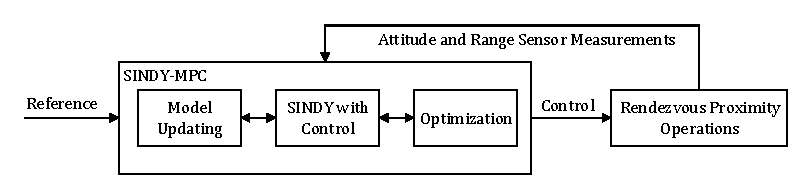
\includegraphics[width=5.0in]{Figures/SINDY_MPC.pdf}
	\caption{System identification using SINDY within MPC, for RPO.}
	\label{fig:SINDY_MPC}
\end{figure}

The diagram shown in Figure \ref{fig:SINCYC} shows the process of solving for the system model. First, to present the identification problem in solvable way, one must first collect measurement data from the unknown dynamic system represented by
\begin{equation}
\label{eq:unknown_dyn}
\dot{X} = \Xi\Theta(X,U).
\end{equation}
Then the control developer must select a library of candidate functions that will be used to build $\Theta(X,U)$. The candidate terms can include polynomial, trigonometric, and other nonlinear functions of states $X$ and inputs $U$. One then substitutes in the measured data into $\dot{X}$ and $\Theta$ in Equation \eqref{eq:unknown_dyn}, and we choose $\Xi$ such that we have the minimum number of terms that effectively describe our dynamics. In other words, we solve for  
\begin{equation}
\label{eq:sparse_reg}
\xi_k = \arg\,\min\limits_{\xi_k}\frac{1}{2}||\dot{X}_k-\xi_k\Theta(X,U)||^2+\lambda||\xi_k||, 
\end{equation}
where subscript $k$ in $\dot{X}_k$ and $\xi_k$ represents the $k$\textsuperscript{th} term of $\dot{X}$ and $\Xi$, and $\lambda$ is chosen to balance between model complexity and accuracy. Once the optimal $\xi_k$ terms are found, they are  directly used to model the unknown system within MPC.

\begin{figure}[h!]
	\centering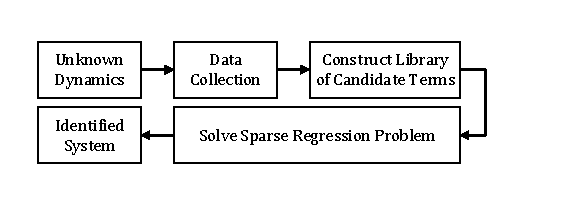
\includegraphics[width=3.64in]{Figures/SINDYC.pdf}
	\caption{Process of using measured data to identify nonlinear system dynamics.}
	\label{fig:SINCYC}
\end{figure}

\bibliographystyle{AAS_publication}   % Number the references.
\bibliography{references}   % Use references.bib to resolve the labels.

\end{document}
